% Options here are passed to the article class.
% Most common options: 10pt, 11pt, 12pt
\documentclass[10pt]{datasheet}

% Input encoding and typographical rules for English language
\usepackage[utf8]{inputenc}
\usepackage[english]{babel}
\usepackage[english]{isodate}

% tikz is used to draw images in this example, but you can
% also use \includegraphics{}.
\usepackage{graphicx}

% These define global texts that are used in headers and titles.
\title{EC06: Item to Binary Encoder With Safety Features}
\author{Obi}
\tags{encoders, safety-features}
\date{25 December 2023}
\revision{Revision 1}
\begin{document}
\maketitle

\section{Features}

\begin{itemize}
\item{10 bit encoding with up to 1024 codes}
\item{Easily accessible coding chests}
\item{Safety features to prevent errors}
\item{Dry fire protection and detection}
\end{itemize}

\section{Applications}

\begin{itemize}
\item{Encoding items}
\end{itemize}

\section{General Description}
The EC06 Item to Binary Encoder With Safety Features is a 10 bit encoder with up to 1024 codes. It has safety features to prevent errors, namely dry fire protection and detection. It uses bit grouping to reduce the amount of chests needed for encoding. \href{https://www.youtube.com/watch?v=1jVHZONWJmg}{Youtube video}

\vfill\break

\begin{figure}[h]
    \centering
    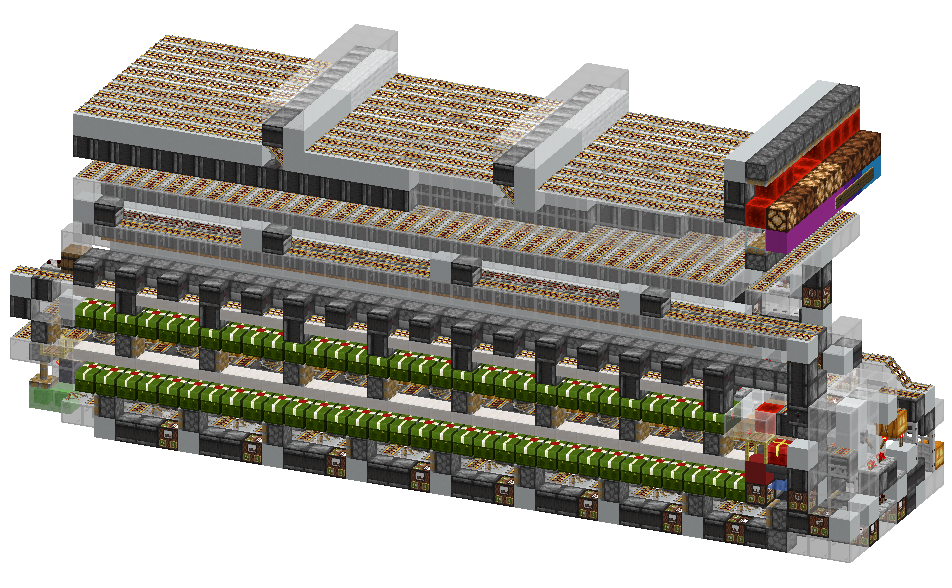
\includegraphics[width=0.48\textwidth]{coderpic.png}
    \caption{\centering Item to Binary Encoder With Safety Features}
\end{figure}

% For wide tables, a single column layout is better. It can be switched
% page-by-page.
\onecolumn

\section{Device Specifications}

\begin{table}[h]
    \caption{Inputs}
    \begin{tabularx}{\textwidth}{l | c | X}
        \thickhline
        \textbf{Name} & \textbf{Range} & \textbf{Description} \\
        \hline
        Box input & Box Item & Single-type box with items for encoding. \\
        \thickhline
\end{tabularx}
\end{table}

\begin{table}[h]
    \caption{Outputs}
    \begin{tabularx}{\textwidth}{l | c | X}
        \thickhline
        \textbf{Name} & \textbf{Range} & \textbf{Description} \\
        \hline
        Box output & Box Item & Outputs the inputted box timed with the code. \\
        \hline
        Code signal & Code & Outputs a binary code corresponding to the mapped item. \\
        \hline
        Error & 0-1 & Outputs redstone signal if error is detected. \\
        \hline
        \thickhline
\end{tabularx}
\end{table}

\begin{table}[h]
    \caption{Device Specifications}
    \begin{tabularx}{\textwidth}{l | c c c | c | X}
        \thickhline
        \textbf{Parameter} & \textbf{Min.} & \textbf{Typ.} & \textbf{Max.} &
        \textbf{Unit} & \textbf{Conditions} \\
        \hline
        Throughput  & 175 & - & - & gt & Normal Usage \\
        \hline
        Latency    & 119 & - & - & gt & From input to code output. \\
        \hline
        MC Version & 1.16 & 1.17.1 & - & MCV & Latest version at time of writing: 1.20.4\\
        \hline
        Dimensions & & 12 x 19 x 40 & & Blocks & \\
        \thickhline
\end{tabularx}
\end{table}
\newpage
\section{Testing Data}
\begin{table}[h]
\caption{Executed Tests}
\begin{tabularx}{\textwidth}{l | X}
    \thickhline
    \textbf{Test} & \textbf{Result} \\
    \hline
    Encoding test & Device was able to encode properly with random input. \\
    \thickhline
\end{tabularx}
\end{table}

\section{Download Information}
\begin{table}[h]
    \caption{Download Information}
    \begin{tabularx}{\textwidth}{l | l | l | X}
        \thickhline
        \textbf{Identifier} & \textbf{MC} & \textbf{File} & \textbf{Description} \\
        \hline
        EC06 & 1.17.1 & \href{https://github.com/Soontech-Annals/Archive/blob/8413f90a054b6c415703bae02badeba7541344f6/Archive/encoders/EC06\%20Item\%20to\%20Binary\%20Encoder\%20With\%20Safety\%20Features/EC06\_Item\_to\_Binary\_Encoder\_With\_Safety\_Features.zip?raw=1}{EC06\_Item\_to\_Binary\_Encoder\_With\_Safety\_Features.zip} & WDL of device. \\
        \hline
        EC06 & 1.17.1 & \href{https://github.com/Soontech-Annals/Archive/blob/8413f90a054b6c415703bae02badeba7541344f6/Archive/encoders/EC06\%20Item\%20to\%20Binary\%20Encoder\%20With\%20Safety\%20Features/EC06\_Item\_to\_Binary\_Encoder\_With\_Safety\_Features.litematic?raw=1}{EC06\_Item\_to\_Binary\_Encoder\_With\_Safety\_Features.litematic} & Schematic of device. \\
        \hline
        \thickhline
    \end{tabularx}
\end{table}

\end{document}

